\documentclass[a4paper,12pt,oneside]{article}

% Imported packages
\usepackage[english]{babel}
\usepackage[T1]{fontenc}
\usepackage[utf8]{inputenc}
\usepackage{amssymb}
\usepackage{amsmath}
\usepackage{graphicx}
\usepackage{geometry}
\usepackage{float}
\usepackage{subfigure}
\usepackage{wrapfig}
\usepackage{comment}
\usepackage{hyperref}

% Margin dimensions settings
\geometry{a4paper,top=2cm,bottom=2cm,left=2cm,right=2cm,%
heightrounded,bindingoffset=5mm}

% Enumeration settings
\renewcommand{\thesection}{\arabic{section})}
\renewcommand{\thesubsection}{\arabic{section}\alph{subsection})}

% Included images path
\graphicspath{{Images/}}

% Document information
\title{Fundamentals of Vibration Analysis and Vibroacoustics \\
Module 1 - Fundamentals of Vibration Analysis \\
Assignment 1 - One-degree-of-freedom systems}
\author{Bombaci Nicola 10677942 \\
Fantin Jacopo 10591775 \\
Intagliata Emanuele 10544878}
\date{April 2020}


\begin{document}

\maketitle

\vspace{60pt}

\section*{System schematic and parameters}

\begin{wrapfloat}{figure}{I}{0pt}
	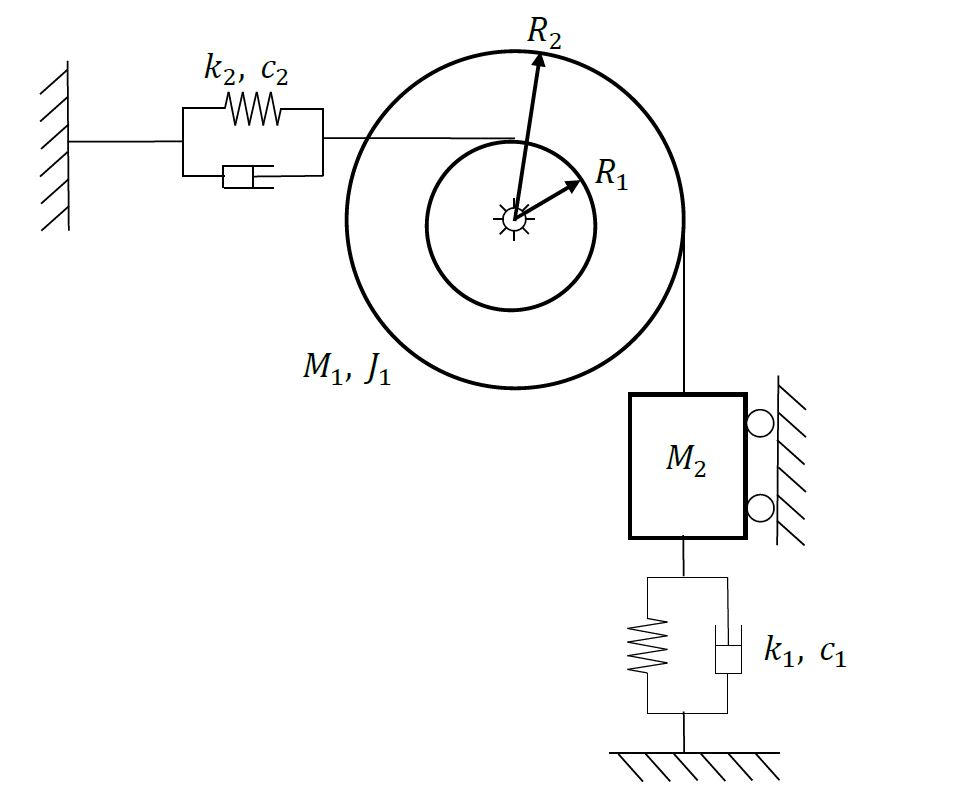
\includegraphics[width=0.7\textwidth]{system_schematic}
\end{wrapfloat}

\[ \begin{split}
	& \begin{cases}
		M_1 = 1 \, \text{kg} \quad \text{,} \quad
			J_1 = 0.005 \, \text{kg m $ \! \! ^2 $} \\
		M_2 = 0.35 \, \text{kg}
	\end{cases} \\[30pt]
	& \begin{cases}
		R_1 = 0.1 \, \text{m} \\
		R_2 = 0.3 \, \text{m}
	\end{cases} \\[30pt]
	& \begin{cases}
		k_1 = 18 \, \text{N/m} \\
		k_2 = 25 \, \text{N/m}
	\end{cases} \\[30pt]
	& \begin{cases}
		c_1 = 0.7 \, \text{Ns/m} \\
		c_2 = 1.2 \, \text{Ns/m}
	\end{cases}
\end{split} \]

\clearpage

\section{Equation of motion}

As a preliminary step, a reference system and sign conventions must be fixed. We chose to follow the commonly employed cartesian axes system, the counterclockwise rotation as the positive one and the spring elongation as the positive variation of the spring length:

\begin{figure}
	\centering
	\subfigure{
		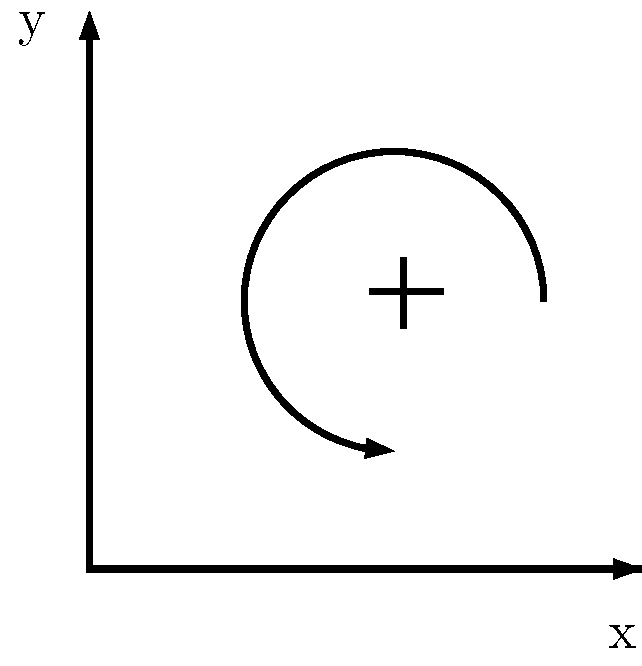
\includegraphics[width=0.15\linewidth]{reference_axes}}
	\hspace{50pt}
	\subfigure{
		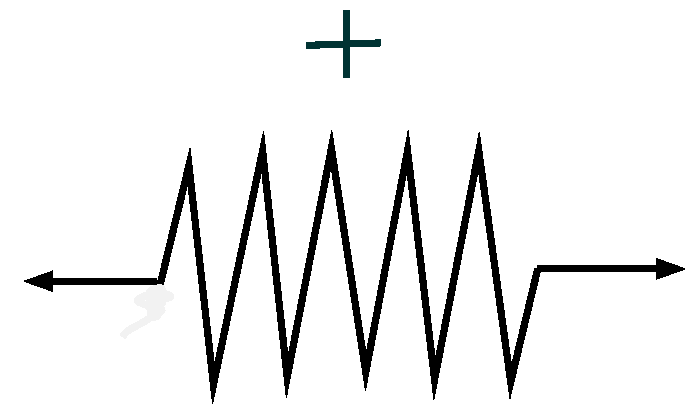
\includegraphics[width=0.15\linewidth]{reference_spring}}
\end{figure}

\subsection{Equation derivation}

\subsubsection*{Step 1: number of degrees of freedom identification}

We can verify the system has one degree of freedom since

\[ \begin{split}
	n_b \cdot 3 ~ \text{DOF} = 6 ~ \text{DOF} & - \\
	2 ~ \text{DOF} & - \quad \text{(hinge)} \\
	2 ~ \text{DOF}  & - \quad \text{(2 rollers)} \\
	1 ~ \text{DOF} & = \quad \text{(string)} \\
	1 ~ \text{DOF}
\end{split} \]

Where $ n_\textup{b} $ is the number of bodies in the system, $ n_\textup{b} = 2 $ in this case. We chose to solve the problem directly using Lagrange equation, so to have one equation only, as the system has one degree of freedom, depending on one independent variable, which we chose to be the disks $ M_1 $ rotation, $ \theta $.

\subsubsection*{Step 2: energy terms definition}

\[ E_\textup{k} = \frac{1}{2} \, J_1 \, \omega_1^2 + \frac{1}{2} \, M_2 \, v_2^2 \]

\[ \begin{split}
	V_\textup{e} = \frac{1}{2} \, k_1 \, \Delta l_1^2 +
		\frac{1}{2} \, k_2 \, \Delta l_2^2 \, \text{;} \quad
		V_\textup{g} = M_2 \, g \, h_2 \\
	\Rightarrow ~ V = V_\textup{e} + V_\textup{g} =
		\frac{1}{2} \, k_1 \, \Delta l_1^2 + \frac{1}{2} \, k_2 \, \Delta l_2^2
		+ M_2 \, g \, h_2
\end{split} \]

\[
	D = \frac{1}{2} \, c_1 \, \dot{\Delta l_1}^2 +
		\frac{1}{2} \, c_2 \, \dot{\Delta l_2}^2
\]

Because the assignment's requests define external forces to compute the system's forced motion later on, we're assuming a vertical force $ F(t) $, directed upward, applied on $ M_2 $, so that we'll find a positive Lagrangian component.

\[ \delta W = F(t) \, \delta y_2 \]

\subsubsection*{Step 3: physical variables as functions of independent ones}

The independent variable $ \theta $ is chosen to be the one variable we need to describe the motion.

\[ \begin{split}
	& \omega_1 = \dot{\theta} \\
	& v_2 = \dot{y_2} = \omega_1 \, R_2 = \dot{\theta} \, R_2 \\
	& \dot{\Delta l_1} = \dot{\theta} \, R_2 \quad \text{(Rivals theorem)}
		~ \Rightarrow ~ \Delta l_1 = \theta \, R_2 \\
	& \dot{\Delta l_2} = - \dot{\theta} \, R_1 \quad \text{(Rivals theorem)}
		~ \Rightarrow ~ \Delta l_2 = - \theta \, R_1 \\
	& h_2 = y_2 = \theta \, R_2
		\quad \text{(gravitational potential level $ = 0 $ at equilibrium point)} \\
	& \delta y_2 = \delta \theta \, R_2 \\
\end{split} \]

\subsubsection*{Step 4: resulting equation}

We first need to find the Lagrangian component $ Q_\theta $ of the force $ F(t) $:

\[
	\delta W = Q_\theta \, \delta \theta =
		F(t) \, \delta y_2 = F(t) \, \delta \theta \, R_2 ~ \Rightarrow ~
		Q_\theta = F(t) \, R_2
\]

Then, the equation of motion is

\[ \begin{split}
	\frac{\partial}{\partial t}
		\Bigl(\frac{\partial E_c}{\partial \dot{\theta}}\Bigr) -
		\frac{\partial E_c}{\partial \theta} +
		\frac{\partial V}{\theta} +
		\frac{\partial D}{\partial \dot{\theta}} & = Q_\theta \\[10pt]
	\Rightarrow ~ (J_1 + M_2 \, R_2^2) \,	\ddot{\theta} +
		(c_1 \, R_2^2 + c_2 \, R_1^2)	\dot{\theta} +
		(k_1 \, R_2^2 + k_2 \, R_1^2) \, \theta & = F(t) \, R_2 - M_2 \, g \, R_2
\end{split} \]

The right side of the equation shows a gravitational contribution in terms of torque. Since we know the system is in the static equilibrium position, this contribution doesn't do any work and, therefore, the static preload of the springs already compensates for it. We can include this static preload in the equation considering a new independent variable, $ \bar{\theta} $, which is the independent variable $ \theta $ in the static equilibrium point, called perturbed variable:

\[
	\bar{\theta} = \theta - \theta_\textup{eq} ~ \Rightarrow ~
		\dot{\bar{\theta}} = \dot{\theta} ~ \Rightarrow ~
		\ddot{\bar{\theta}} = \ddot{\theta}
\]

where $ \theta_\textup{eq} $ is a constant that accounts for the static preload, computed at the static ($ \dot{\theta} = 0 $) equilibrium ($ \ddot{\theta} = 0 $) position:

\[ \begin{split}
	(k_1 \, R_2^2 + k_2 \, R_1^2) \, \theta_\textup{eq} =
		F(t) \, R_2 - M_2 \, g \, R_2 \\
	\Rightarrow ~ \theta_\textup{eq} =
		\frac{F(t) \, R_2 - M_2 \, g \, R_2}{(k_1 \, R_2^2 + k_2 \, R_1^2)}
\end{split} \]

We consider the force as composed by a constant value and a variable one $ F(t) = F_\textup{eq} + F \, cos(\Omega \, t + \varphi) $. In the static equilibrium position, the variable part of the force is null, so we just have that $ F(t) = F_\textup{eq} $:

\[
	\theta_\textup{eq} =
		\frac{F_\textup{eq} \, R_2 - M_2 \, g \, R_2}{(k_1 \, R_2^2 + k_2 \, R_1^2)}
\]

The final equation of motion in the equilibrium position is

\begin{equation}
\label{eqn:motion}
	\underbrace{(J_1 + M_2 \, R_2^2)}_
		{\substack{\text{generalized mass} \\ \text{$ m_\textup{g} $}}} \,
		\ddot{\bar{\theta}} +	\underbrace{(c_1 \, R_2^2 + c_2 \, R_1^2)}_
		{\substack{\text{generalized damping} \\ \text{$ c_\textup{g} $}}} \,
		\dot{\bar{\theta}} + \underbrace{(k_1 \, R_2^2 + k_2 \, R_1^2)}_
		{\substack{\text{generalized stiffness} \\ \text{$ k_\textup{g} $}}} \,
		\bar{\theta} = F(t) \, R_2 =
		\underbrace{F \, R_2 \, cos(\Omega \, t + \varphi)}_
		{\substack{\text{generalized force} \\ \text{$ Q_\theta $}}}
\end{equation}

\subsection{Adimensional damping ratio}

\begin{equation}
\label{eqn:damping_ratio}
	\xi = \frac{c_\textup{g}}{c_\textup{cr}} =
		\frac{c_\textup{g}}{2 \, \sqrt{k_\textup{g} \, m_\textup{g}}}
		= \frac{c_1 \, R_2^2 + c_2 \, R_1^2}
		{2 \, \sqrt{(k_1 \, R_2^2 + k_2 \, R_1^2) \, (J_1 + M_2 \, R_2^2)}}
		\approx 0.134
\end{equation}

\subsection{Natural and damped frequency}

\[
	\omega_\textup{n} = \sqrt{\frac{k_\textup{g}}{m_\textup{g}}} =
		\sqrt{\frac{k_1 \, R_2^2 + k_2 \, R_1^2}{J_1 + M_2 \, R_2^2}}
		\approx 7.16 \, \text{rad/s}
\]

\begin{equation}
\label{eqn:damping_factor}
  \alpha = \xi \, \omega_\textup{n} \approx 0.959 \, \text{rad/s}
\end{equation}

\begin{equation}
\label{eqn:damped_frequency}
	\omega_\textup{d} = \sqrt{\omega_n^2 - \alpha^2} \approx 7.09 \, \text{rad/s}
\end{equation}


\section{Free motion of the system}

The system's free motion is described by the general solution to the differential equation of motion, which corresponds to the solution to the homogeneous differential equation associated to \eqref{eqn:motion}:

\[
	m_\textup{g} \, \ddot{\bar{\theta}} + c_\textup{g} \, \dot{\bar{\theta}} +
		k_\textup{g} \, \bar{\theta} = 0
\]

We solved this equation manually, finding the characteristic polynomial roots and summing the two resulting exponential functions, each with one of the two eigenvalues. The solution, plotted below, has the analytic form

\[ \begin{split}
	\bar{\theta}^\textup{free}(t)	&
		= \bar{X}_1 \, e^{\lambda_1 \, t} + \bar{X}_2 \, e^{\lambda_2 \, t} = \\
	& = \bar{X}_1 \, e^{(-\alpha + j \omega_\textup{d}) \, t} +
		\bar{X}_2 \, e^{(-\alpha - j \omega_\textup{d}) \, t} = \\
	& = e^{-\alpha \, t} \, (\bar{X}_1 \, e^{j \omega_\textup{d} \, t} +
		\bar{X}_2 \, e^{- j \omega_\textup{d} \, t})
\end{split} \]

which represents an oscillatory behavior modulated by a decaying exponential, as expected, and where the coefficients $ \bar{X}_1 $ and $ \bar{X}_2 $ are computed starting from the system parameters and the initial conditions according to the following relations:

\[
	\begin{cases}
		\theta_0 = \bar{\theta}^\textup{free}(t = 0) = \bar{X}_1 + \bar{X}_2 \\
		\omega_0 = \dot{\bar{\theta}}^\textup{free}(t = 0) =
			\lambda_1 \, \bar{X}_1 + \lambda_2 \, \bar{X}_2
	\end{cases} ~ \Rightarrow ~
		\begin{cases}
			\bar{X}_1 = \theta_0 - \frac{\omega_0 - \lambda_1 \, \theta_0}
				{\lambda_2 - \lambda_1} \\
			\bar{X}_2 = \frac{\omega_0 - \lambda_1 \, \theta_0}{\lambda_2 - \lambda_1}
		\end{cases}
\]

\subsection{Generic initial conditions}
\label{subs:generic_initial_conditions}

In order for the equation to be computed and represented in a diagram, some initial conditions need to be settled. The shown response in time domain is obtained with these arbitrary initial conditions:

\[ \begin{cases}
	\theta_0 = 2 \, \text{rad} \\
	\omega_0 = 16 \, \text{rad/s}
\end{cases} \]

These values allow us for a clearer visualization of the motion, and an easier distinction between the transient and the steady-state behavior.

\begin{figure}[H]
	\hspace{-30pt}
	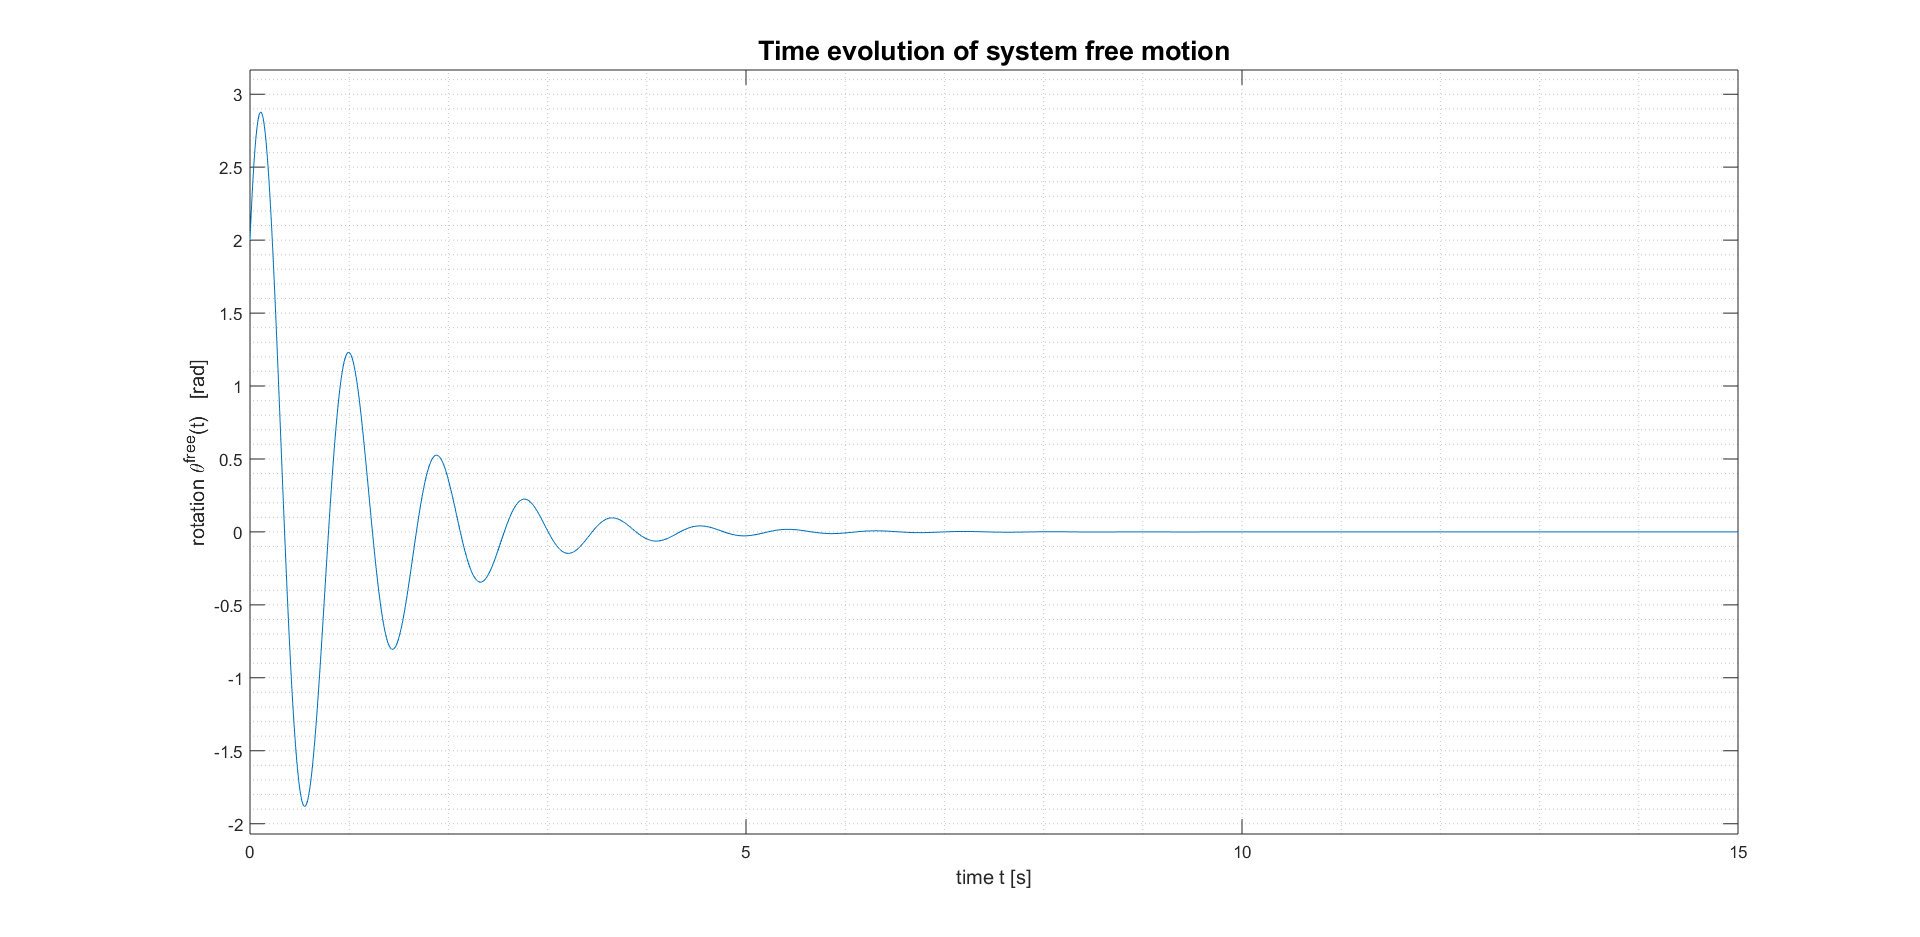
\includegraphics[scale=0.35]{free_time_response}
\end{figure}

\vspace{50pt}

\subsection{Halved adimensional damping ratio}

The system resulting from halving $ \xi $ is equivalent to that obtained by halving the damping coefficient $ c_\textup{g} $, in conformity with \eqref{eqn:damping_ratio}. As a consequence, the system shows a much lightlier damped free oscillation, and the time leading to an almost completely damped away motion is doubled. In fact, if $ t_0 $ and $ t'_0 $ are the earliest time instants for which the oscillation may be considered as over in the previous case and with halved $ \xi $ respectively (we assumed $ 10^{-6} $ times the initial amplitude), and remembering that, if $ \xi $ is halved, then $ \alpha $ is halved too according to \eqref{eqn:damping_factor}:

\[ \begin{split}
	e^{-\alpha \, t_0} = 10^{-6} ~ \Rightarrow ~
		t_0 & = \frac{ln(1) - ln(10^6)}{-\alpha} = \\
				& = \frac{ln(10^6)}{\alpha} \approx 14.41 \, \text{s}
\end{split} \]

\[ \begin{split}
	e^{-\frac{\alpha}{2} \, t'_0} = 10^{-6} ~ \Rightarrow ~
		t'_0 & = \frac{ln(1) - ln(10^6)}{-\alpha} = \\
				 & = 2 \, \frac{ln(10^6)}{\alpha} = 2 \, t_0 \approx 28.81 \, \text{s}
\end{split} \]

Assuming the same initial conditions as before, the free response is depicted in the following plot:

\clearpage

\begin{figure}[h]
	\hspace{-70pt}
	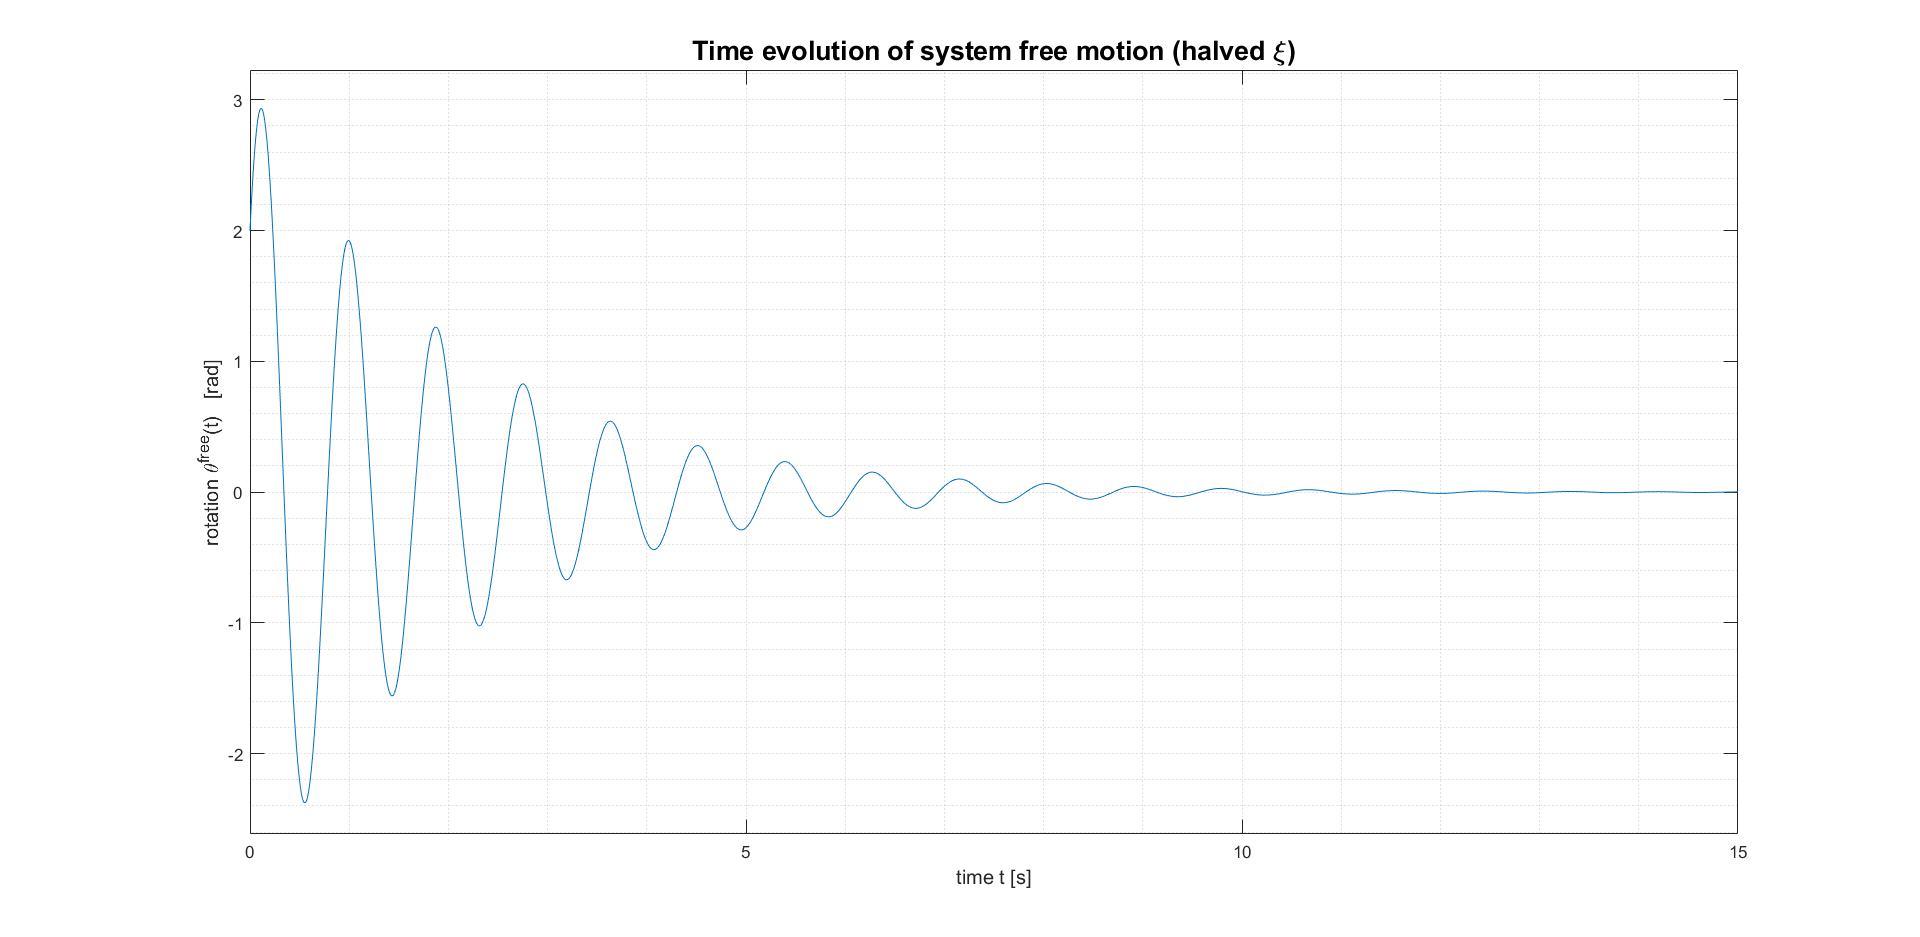
\includegraphics[scale=0.4]{free_time_response_halved_damping_ratio}
\end{figure}

\vspace{50pt}

\subsection{Raised adimensional damping ratio}

Instead, if the damping ratio is increased so that $ \xi > 1 $ holds, the damping coefficient becomes greater than the critical damping coefficient $ c_\textup{cr} $, which means that the system is overdamped. Choosing $ \xi = 1.2 $, we computed the corresponding $ c_\textup{g} $ using \eqref{eqn:damping_ratio} and we solved again the free motion equation, getting a totally analogous solution, except for the fact the exponential functions are not complex anymore, but real. This results in the sum of two decaying exponentials, which is in turn a decaying exponential.

\[
	\bar{\theta}^\textup{free}(t) =
		\bar{X}_1 \, e^{\lambda_1 \, t} + \bar{X}_2 \, e^{\lambda_2 \, t} =
		\bar{X}_1 \, e^{-\alpha_1 \, t} + \bar{X}_2 \, e^{-\alpha_2 \, t}
\]

We can appreciate the absence of vibration due to the absence of a couple of complex conjugate roots in the characteristic equation solution.

\clearpage

\begin{figure}[h]
	\hspace{-70pt}
	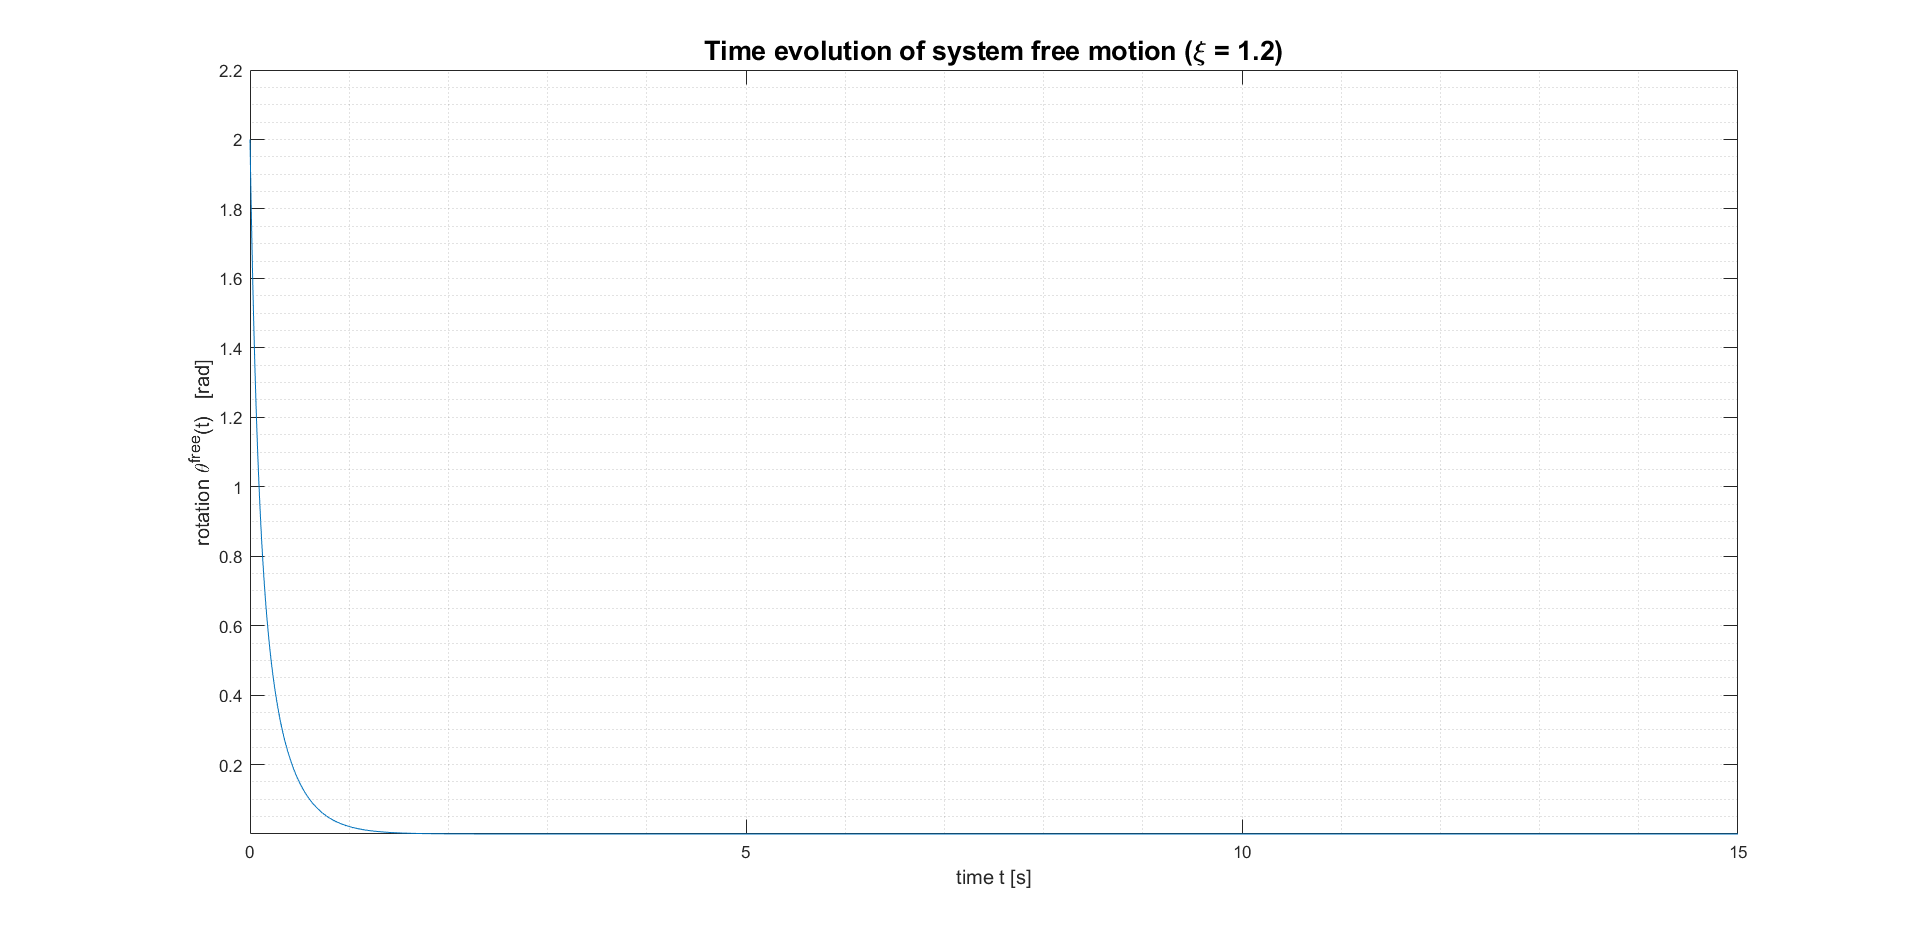
\includegraphics[scale=0.4]{free_time_response_overdamped}
\end{figure}

\section{Forced motion of the system}

\subsection{Frequency Response Function}
\label{subs:frf}

We now come to consider the system as excited by an external torque $ \tau(t) = T \, e^{j \Omega \, t} $, with unitary modulus and applied to the discs counterclockwise: the Frequency Response Function (FRF) of the system is, by definition, the response in terms of amplitude and phase shift (with respect to the applied generalized force itself) of the forced vibration of the independent variable we're considering to an external harmonic excitation whose virtual displacement has a 1x1 Jacobian equal to $ 1 $. This excitation is, in our case, a torque.

First, the FRF has been computed from the system parameters: specifically, in this case, it's defined as the ratio between the complex function embedding the steady-state discs rotation's amplitude and phase, which is a function of the forcing frequency, and the amplitude of the applied torque's oscillation.

\[
	H(\Omega) = \frac{\tilde{\bar{\Theta}}(\Omega)}{T} =
		\frac{1}{m_\textup{g} \, \Omega^2 - j c_\textup{g} \, \Omega + k_\textup{g}}
\]

We're requested to apply it in three different cases.

\subsubsection*{Case 1: generic initial conditions}

In this first case, we're plotting the FRF assuming the system parameters are the given ones, which we started with. Notably, a peak (absolute maximum) in the magnitude diagram corresponds to the natural damped frequency $ \omega_\textup{d} $ of the system, computed at \eqref{eqn:damped_frequency}, which is reflected in the phase diagram in a $ -\pi $ jump.

\clearpage

\begin{figure}[h]
	\hspace{-70pt}
	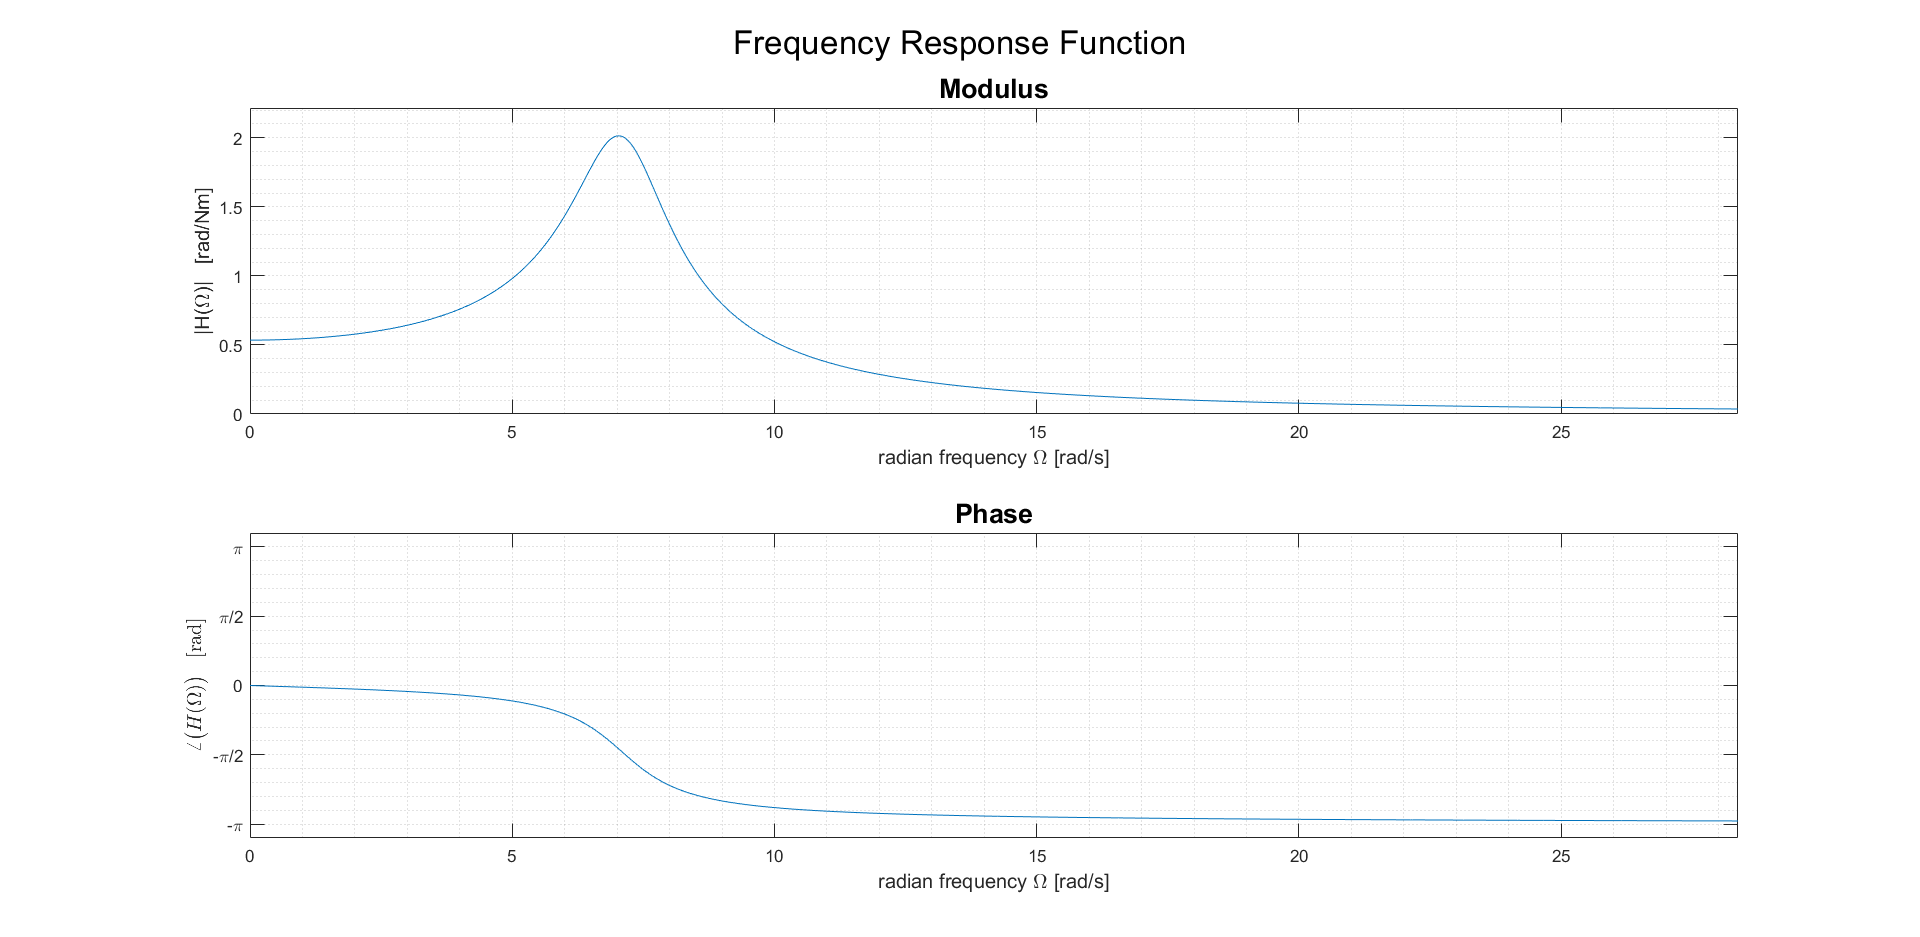
\includegraphics[scale=0.4]{frf}
\end{figure}

\vspace{-5pt}

\subsubsection*{Case 2: halved adimensional damping ratio}

Considering half the damping ratio, we expect the system to be closer to the ideal undamped case, which means that the peak in the modulus diagram is going to be sharper than in the previous case (getting closer to the asymptotic behavior typical of the undamped system) and the phase jump suddener in the phase diagram (getting closer to the ideal perfectly vertical jump of the undamped case). It is worthy to say also the natural damped frequency changes, in accordance with relation \eqref{eqn:damped_frequency}: in particular, its value decreases proportionally to the damping factor $ \alpha $, so the higher the damping, the lower the damped frequency, the more the peak moves to the left in the modulus plot.

\begin{figure}[H]
	\hspace{-70pt}
	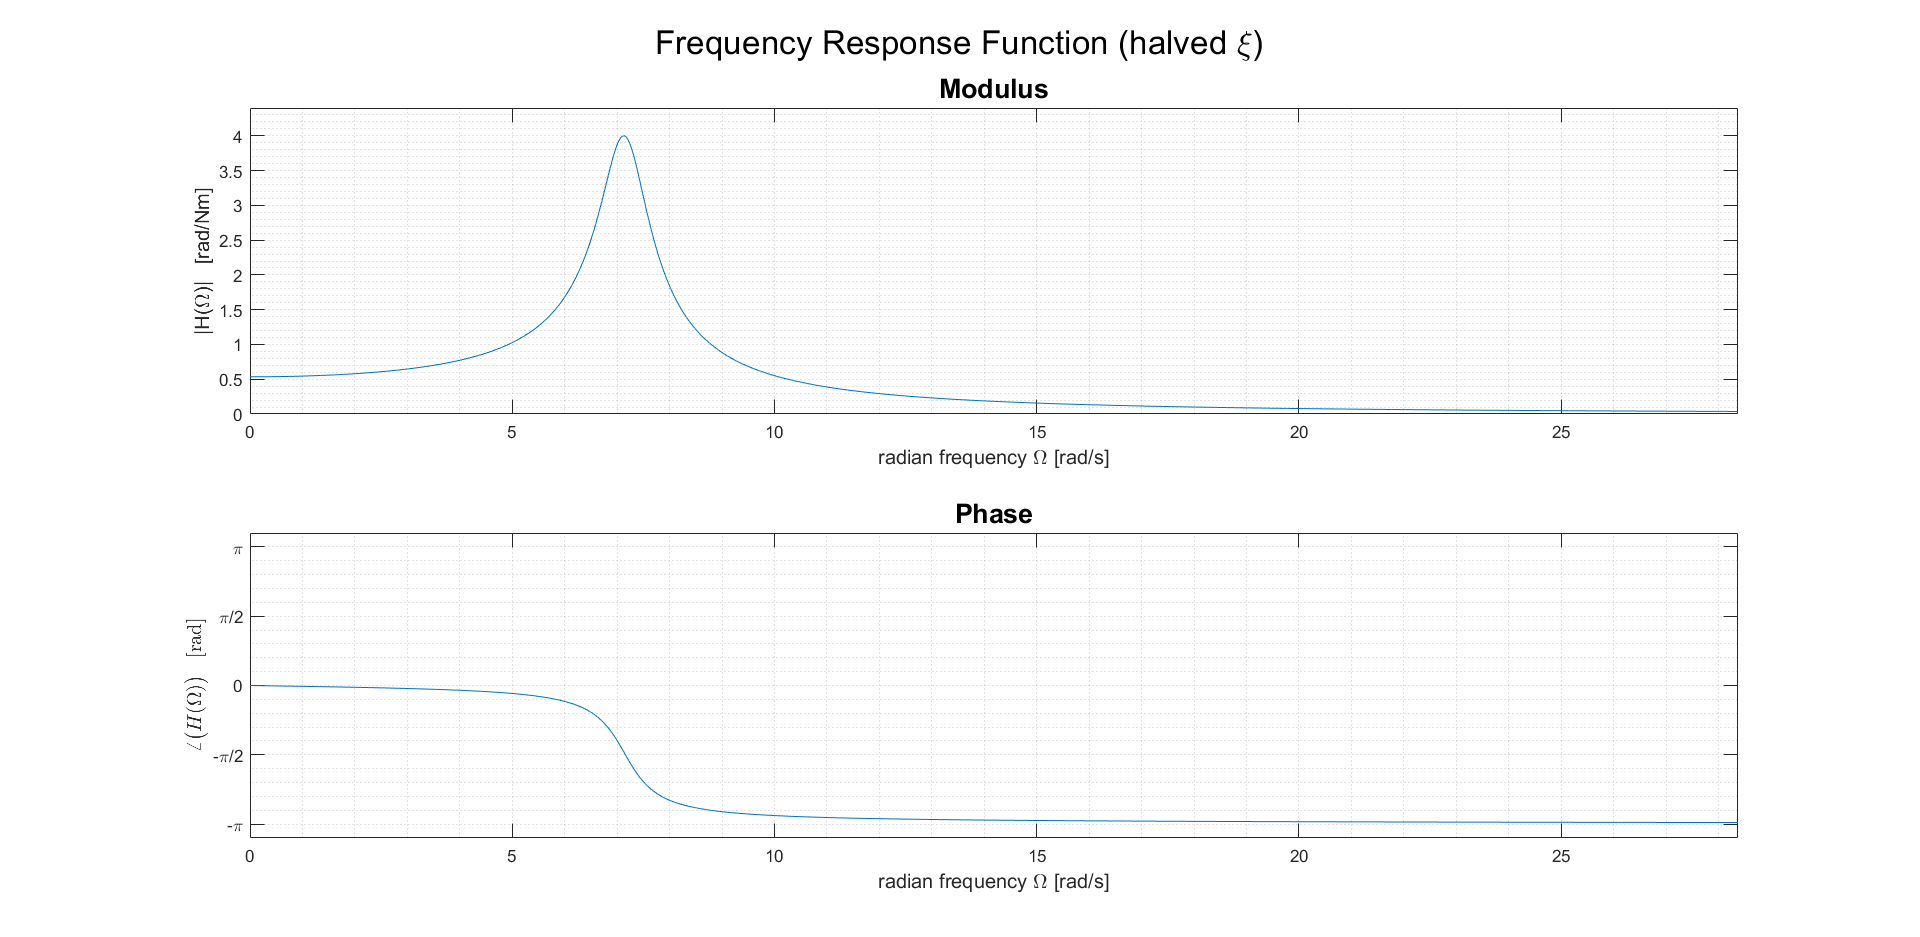
\includegraphics[scale=0.4]{frf_halved_damping_ratio}
\end{figure}

\subsubsection*{Case 3: raised adimensional damping ratio}

In this third case, the adimensional damping ratio is set to $ \xi = 1.2 $, so we find ourselves in the case of the overdamped system. We're expecting a smooth low-pass-like curve in the amplitude diagram as the damped frequency doesn't appear in the analytic formula of the response in time domain, i.e. the system's free motion does not oscillate, so the FRF shape is not depending on the natural frequency of the system. We might notice that the maximum steady-state oscillation amplitude is found for $ \Omega = 0 $, i.e. for a constant external force.

\begin{figure}[H]
	\hspace{-70pt}
	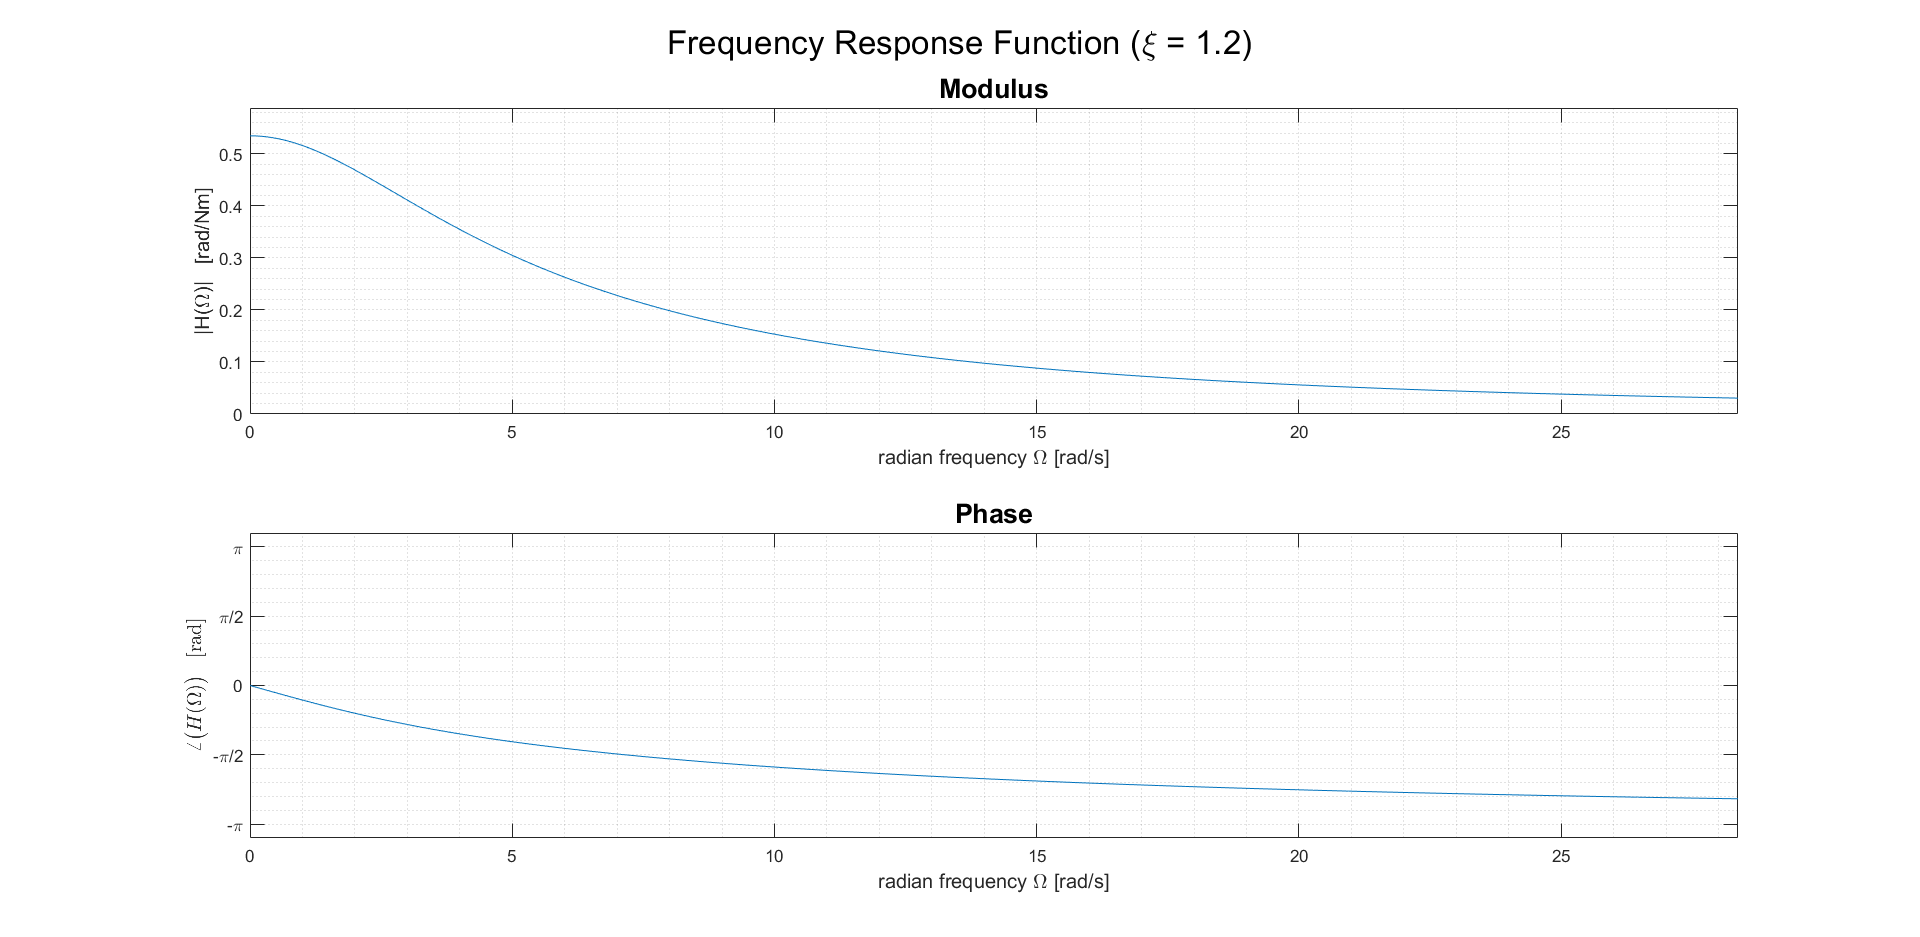
\includegraphics[scale=0.4]{frf_overdamped}
\end{figure}

\vspace{30pt}

\subsection{Complete time response of the system}

The system's complete response is composed by its free response and its forced response, summed together. The former is the one obtained in \ref{subs:generic_initial_conditions}. For the latter, the input force to the system is considered to be a harmonic force applied to body 2, oriented in the vertical direction (we chose the verse to be upward, as it's not specified by the assignment) and made up by a single sinusoidal wave:

\[ F(t) = A \, \cos(2 \pi f_i \, t + \phi) \]

where $ A = 2.5 \, \text{N} $ and $ \phi = \frac{\pi}{3} $. Note that we chose the force for \eqref{eqn:motion} according to the force we're using as the system's input at this point of the assignment. We're considering two different cases for the frequency of this single harmonic component. In the first case

\[
	f_i = f_1 = 0.15 \, \text{Hz} ~ \Rightarrow ~
		\omega_i = \omega_1 = 2 \pi f_1 \approx 0.94 \, \text{rad/s}
\]

while in the second

\[
	f_i = f_2 = 4.5 \, \text{Hz} ~ \Rightarrow ~
		\omega_i = \omega_2 = 2 \pi f_2 \approx 28.27 \, \text{rad/s}
\]

In each case, the steady-state motion has been computed by applying the well-known theoretical result stating the output of a linear time-invariant system is equal to the system input moduated in amplitude and phase by the FRF linking the independent variable with that input force computed for the particular frequency $ \Omega $ of the input:

\begin{equation}
\label{eqn:lti_output}
	x_\textup{out}(t) = |G(j \Omega)| \, F \,
		\cos\Bigl(\Omega t + \varphi + \angle\bigl(G(j \Omega)\bigr)\Bigr)
\end{equation}

The FRF that links the discs rotation with this force is obtained by multiplying the FRF found at \ref{subs:frf} by the correspondent cinematic relationship (i.e. the force's 1x1 Jacobian), which is equal to $ R_2 $ in this case, so the final formula becomes

\[ \begin{split}
	\bar{\theta}(t) & =
		\bar{\theta}^\textup{free}(t) + \bar{\theta}^\textup{forced}(t) = \\
									& = e^{-\alpha \, t} \,
										(\bar{X}_1 \, e^{j \omega_\textup{d} \, t} +
										\bar{X}_2 \, e^{- j \omega_\textup{d} \, t}) +
										|H(\omega_i)| \, R_2 \, \, A \,
										\cos\Bigl(\omega_i \, t + \phi +
										\angle\bigl(H(\omega_i)\bigr)\Bigr)
\end{split} \]

Note that multiplying the FRF by a real positive constant number affects the amplitude only, since the resulting FRF has the amplitude of the system's FRF multiplied by that constant, and the phase of the system's FRF added to the constant's phase, which is zero.

We took the liberty of taking into account an additional case, where the external force frequency nearly matches the system's damped frequency, to check whether the amplitude of the resulting oscillation in steady-state is actually much larger than in the previous cases:

\[
	\omega_i = \omega_3 = 7 \, \text{rad/s} ~ \Rightarrow ~
		f_i = f_3 = \frac{\omega_3}{2 \, \pi} \approx 1.11 \, \text{Hz}
\]

The system's complete responses over time for each of the three cases are visualized in the following diagram. Notably enough, in the first $ 4 \, s $ of the motion, the transient greatly exhibits (much more than the respective forcing frequencies) the system's damped frequency even in the case the forcing frequency is not close to it.

\begin{figure}[h]
	\hspace{-70pt}
	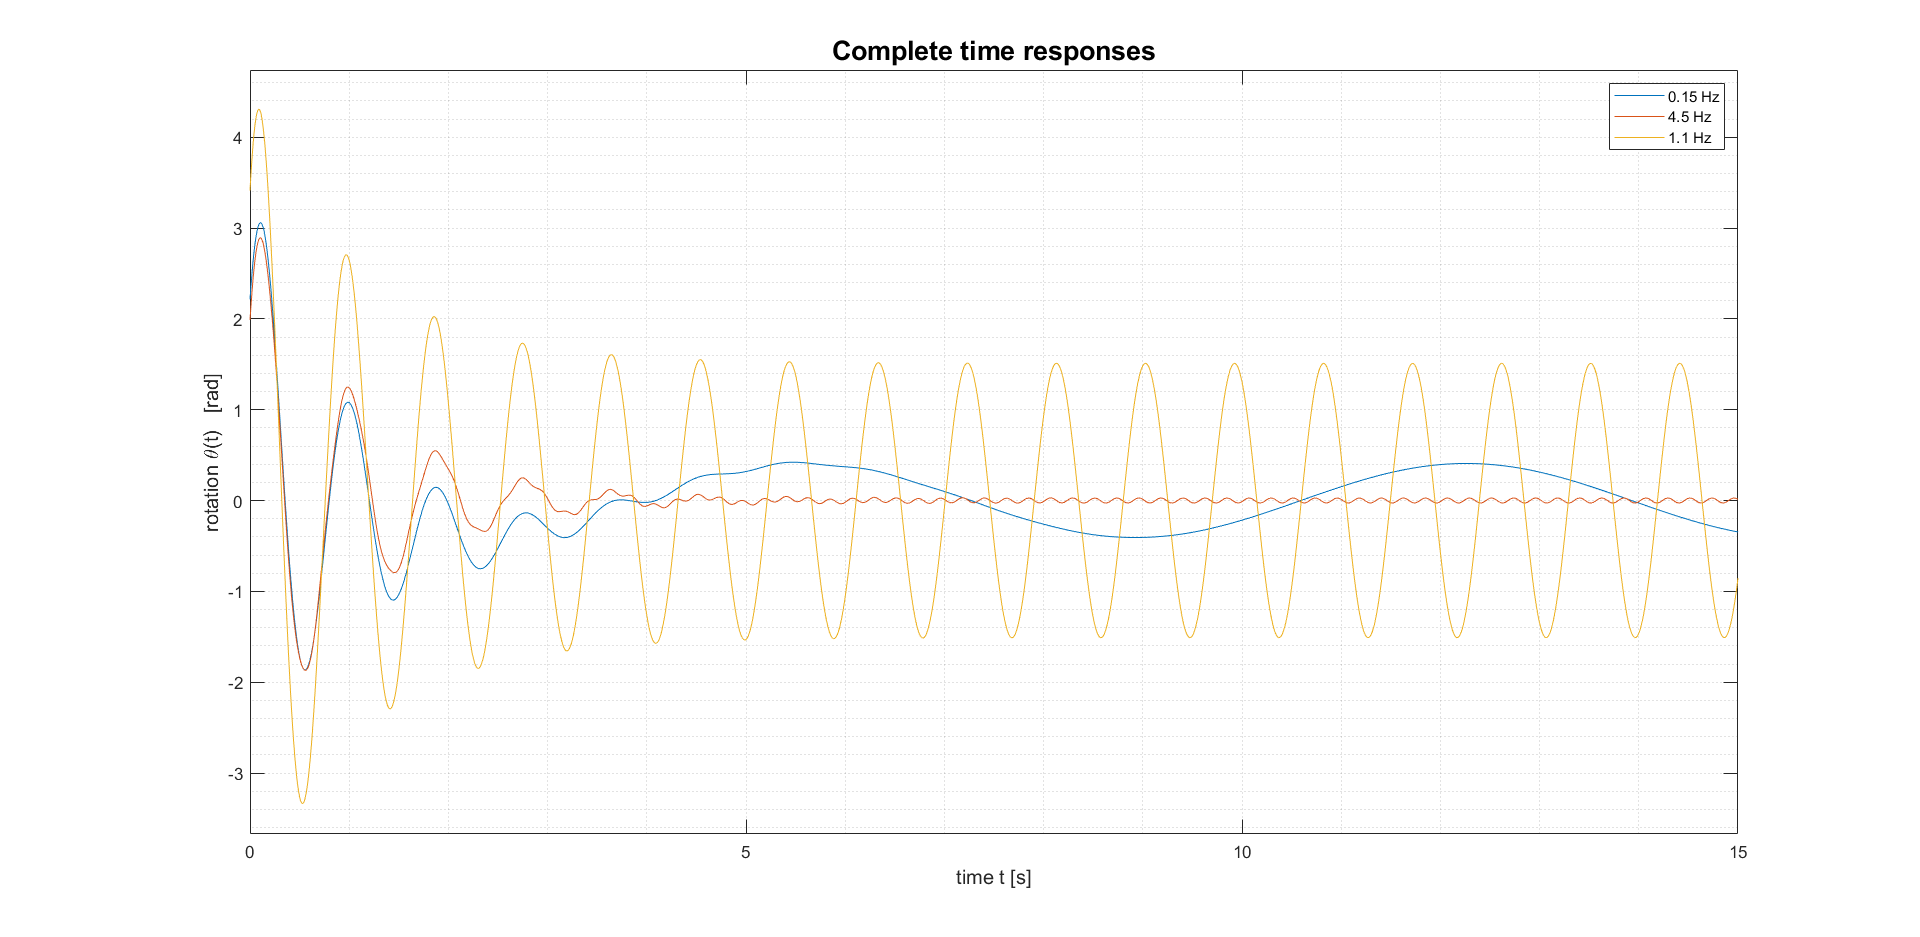
\includegraphics[scale=0.4]{complete_time_responses}
\end{figure}

\clearpage

\subsection{Forced response of the system (steady-state)}

Finally, let's consider this time a complex force composed by three harmonic components as system input and applied as for the previous analysis case:

\[ F(t) = \sum_{k=1}^3 B_k \, \cos(2 \pi f_k \, t + \phi_k) \]

with $ B_1 = 1.2 \, \text{N} $, $ B_2 = 0.5 \, \text{N} $, $ B_3 = 5 \, \text{N} $, $ f_1 = 0.1 \, \text{Hz} $ ($ \omega_1 = 0.63 \, \text{rad/s} $), $ f_2 = 0.6 \, \text{Hz} $ ($ \omega_2 = 3.77 \, \text{rad/s} $), $ f_3 = 3.3 \, \text{Hz} $ ($ \omega_3 = 20.73 \, \text{rad/s} $), $ \phi_1 = \frac{\pi}{4} $, $ \phi_2 = \frac{\pi}{5} $ and $ \phi_3 = \frac{\pi}{6} $. The external force and the forced vibration of the system are analyzed both in time and in frequency domain. For analyzing the forced response, the superposition principle has been employed: using equation \eqref{eqn:lti_output}, we computed the system forced response for each of the individual harmonic components that constitute the oscillating input. We then summed together the three partial forced responses to get the total steady-state response of the system. To validate the resut, we compared the spectrums with the Fast Fourier Transforms of the two time-domain signals making use of the relative Matlab function. As we may see, the amplitude spectra computed by means of FFT, scaled by the FFT length, qualitatively coincide with the ones we constructed showing peaks in correspondence to the same frequencies.

As the external force is concerned, we can easily identify the three sinusoidal components that build it up in time domain, while the spectrum simply displays the given data in terms of amplitude, frequency and phase shift. As for the system's forced vibration, we are again able to tell the three frequency components apart in the time-domain response. Furthermore, we can observe how different the weights of these three components are in the forced response, with respect to the input force: the low frequencies are the most emphasized, while the highest one is attenuated a big deal. This is due to the fact the original amplitudes for each cosine function in the external force are multiplied by the modulus of the corresponding Frequency Response Function computed for the frequency of the cosine functions itself, whereas the particular shape of the waveform is determined by the sum between the original phase shifts for each component with the phase value of the same FRF evaluated for the corresponding frequencies.

\begin{figure}
	\hspace{-70pt}
	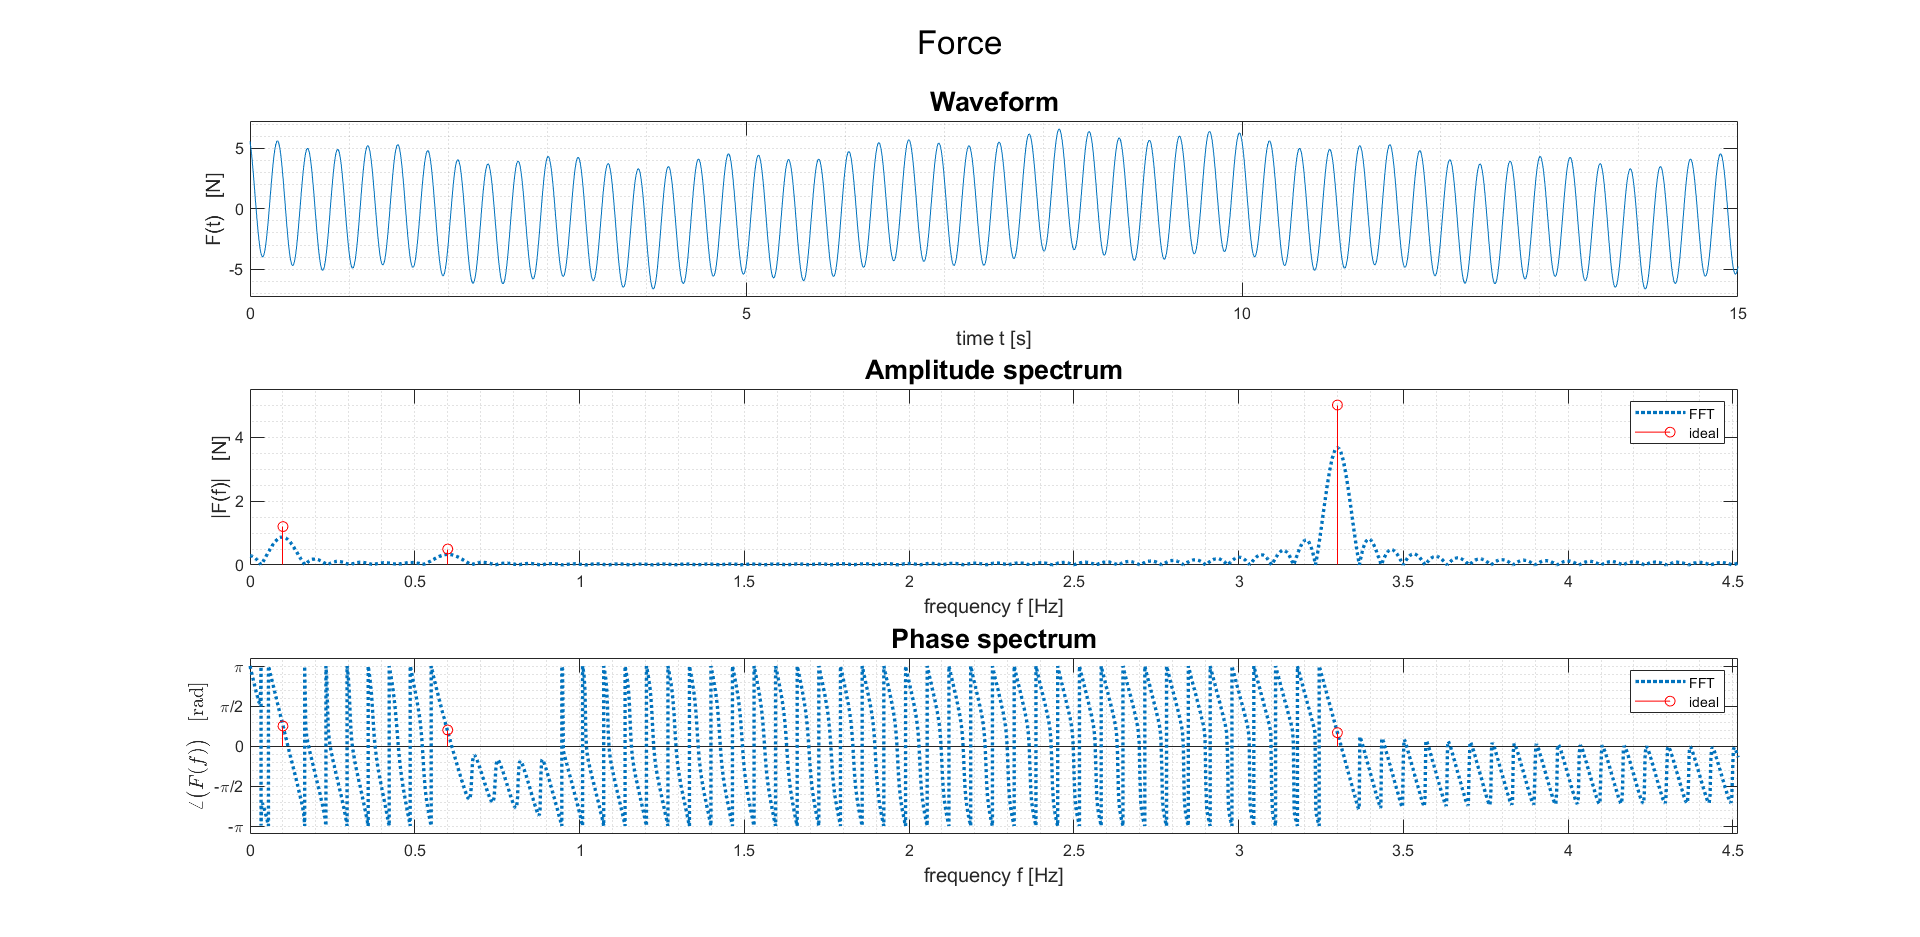
\includegraphics[scale=0.4]{force}
\end{figure}

\begin{figure}
	\hspace{-70pt}
	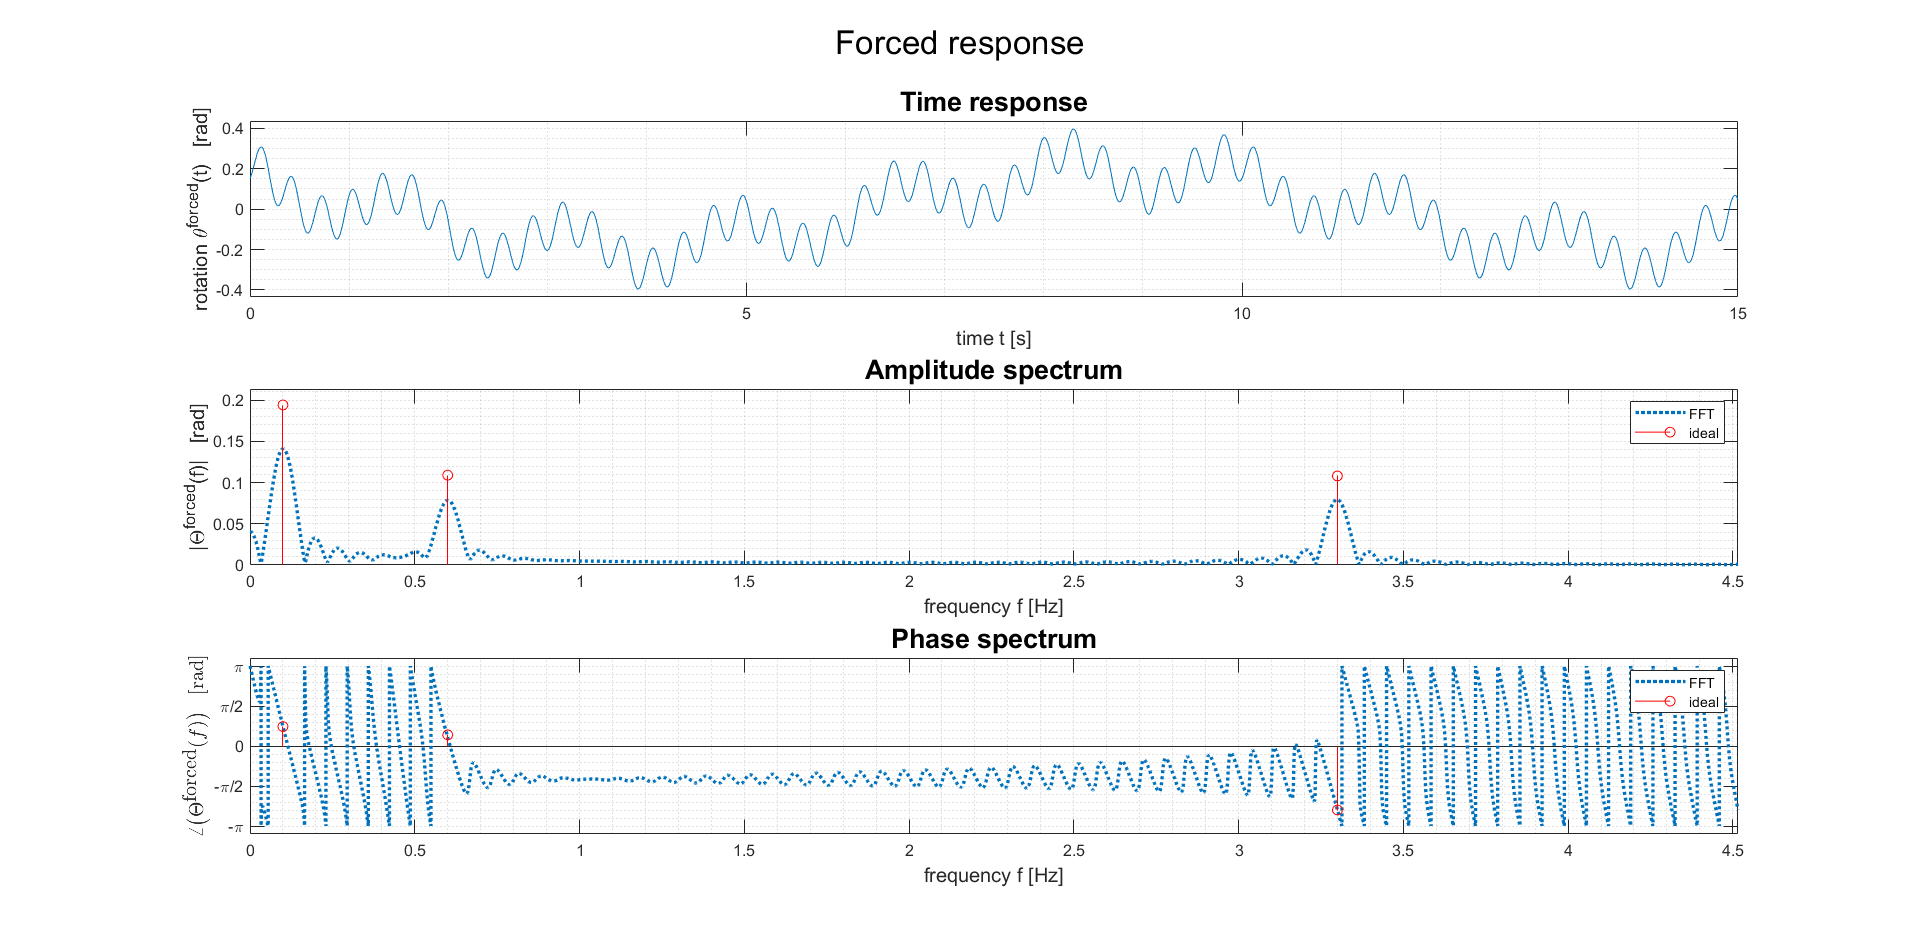
\includegraphics[scale=0.4]{forced_response}
\end{figure}


\end{document}